% Drawing 86/02-1 -- folder 86, batch 02, archive page 22 (PDF page 23).
% Transcription: à gauche, un dessin de l'icosaèdre en perspective, arêtes cachées en pointillé ; sommets marqués $u_1$, $w_1'$, $u'$, $v_1'$, $w$, $v$, $v_1$, $w_1$, $u = s$, $u_1'$, $w'$, $v'$ ; un triangle fondamental hachuré, de sommet $s$, porte sur ses côtés les marques $\sigma_0$, $\sigma_1$, $\sigma_2$
% Kind: icosahedron in perspective. Method 3 (encoded, rendered from the data). Status: ok.
% Notes: Icosahedron with its hidden edges dashed; vertices u_1, w_1', v_1', v_1, w_1, u_1' on the outline, w, v, u = s in front, u', v', w' behind. Encoded as polyhedron/1 with the labels of the page (u=s for the front vertex); the 12 dashed edges are read from scattered dashes and checked against the icosahedron (every vertex of degree 5). The hatched fundamental triangle with apex s carries sigma_0, sigma_1, sigma_2 on its sides.
% Coordinates: 1 unit = 1 mm = 1/100 of the crop width (bbox in page fractions: [0.18, 0.1, 0.45, 0.33]).
% Redrawn by Claude (claude-opus-5-5), issue #73, 2026-11-07; not checked by a human; not compiled (no TeX in the session).
% Rights: reproduces part of the work -- behind RENDER_TRANSCRIPTS, never published by itself.
\documentclass[tikz,border=3pt]{standalone}
\usepackage{amsmath,amssymb}
\usetikzlibrary{patterns,arrows.meta}
\tikzset{pencil/.style={black!45}, struck/.style={black!35}, mark/.style={circle,draw,inner sep=1.3pt}, pt/.style={circle,fill,inner sep=0.9pt}, opt/.style={circle,draw,fill=white,inner sep=1.1pt}}
\begin{document}
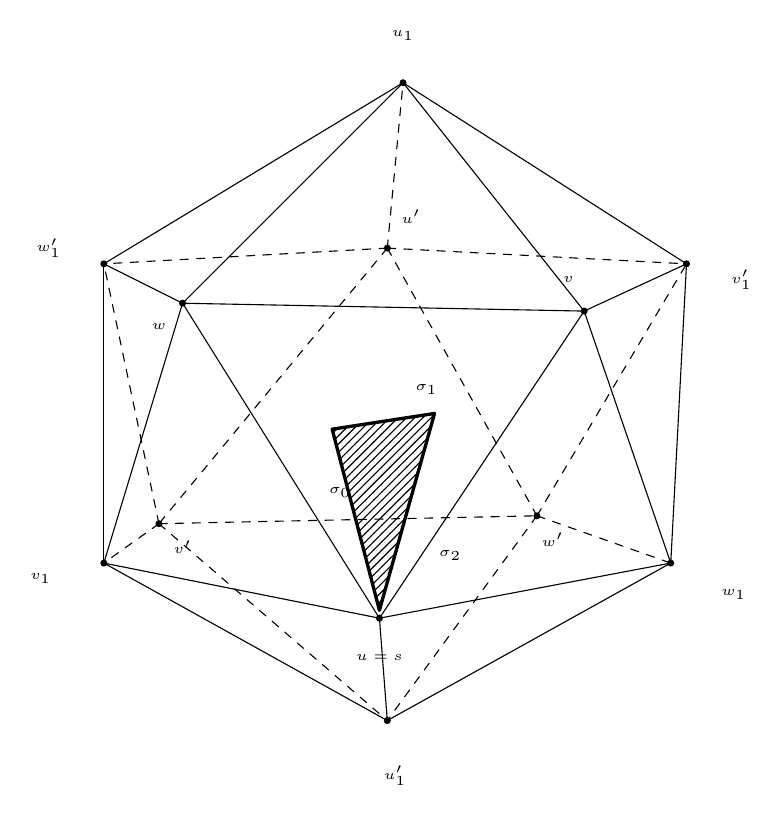
\begin{tikzpicture}[x=1mm,y=1mm,line cap=round,line join=round,font=\scriptsize]
\draw (52,-19) -- (14,-42);
\draw (14,-42) -- (14,-80);
\draw (14,-80) -- (50,-100);
\draw (50,-100) -- (86,-80);
\draw (86,-80) -- (88,-42);
\draw (88,-42) -- (52,-19);
\draw (52,-19) -- (24,-47);
\draw (52,-19) -- (75,-48);
\draw (24,-47) -- (75,-48);
\draw (24,-47) -- (14,-42);
\draw (24,-47) -- (14,-80);
\draw (75,-48) -- (88,-42);
\draw (75,-48) -- (86,-80);
\draw (49,-87) -- (24,-47);
\draw (49,-87) -- (75,-48);
\draw (49,-87) -- (14,-80);
\draw (49,-87) -- (86,-80);
\draw (49,-87) -- (50,-100);
\draw[dashed] (50,-40) -- (52,-19);
\draw[dashed] (50,-40) -- (14,-42);
\draw[dashed] (50,-40) -- (88,-42);
\draw[dashed] (50,-40) -- (21,-75);
\draw[dashed] (50,-40) -- (69,-74);
\draw[dashed] (21,-75) -- (14,-42);
\draw[dashed] (21,-75) -- (14,-80);
\draw[dashed] (21,-75) -- (50,-100);
\draw[dashed] (21,-75) -- (69,-74);
\draw[dashed] (69,-74) -- (88,-42);
\draw[dashed] (69,-74) -- (86,-80);
\draw[dashed] (69,-74) -- (50,-100);
\node[pt] at (52,-19) {};
\node[pt] at (14,-42) {};
\node[pt] at (88,-42) {};
\node[pt] at (14,-80) {};
\node[pt] at (86,-80) {};
\node[pt] at (50,-100) {};
\node[pt] at (24,-47) {};
\node[pt] at (75,-48) {};
\node[pt] at (49,-87) {};
\node[pt] at (50,-40) {};
\node[pt] at (21,-75) {};
\node[pt] at (69,-74) {};
\fill[pattern=north east lines] (49,-86) -- (43,-63) -- (56,-61) -- cycle;
\draw[very thick] (49,-86) -- (43,-63) -- (56,-61) -- cycle;
\node[inner sep=1pt] at (44,-71) {\tiny $\sigma_0$};
\node[inner sep=1pt] at (55,-58) {\tiny $\sigma_1$};
\node[inner sep=1pt] at (58,-79) {\tiny $\sigma_2$};
\node[inner sep=1pt] at (52,-13) {\tiny $u_1$};
\node[inner sep=1pt] at (7,-40) {\tiny $w_1'$};
\node[inner sep=1pt] at (95,-44) {\tiny $v_1'$};
\node[inner sep=1pt] at (6,-82) {\tiny $v_1$};
\node[inner sep=1pt] at (94,-84) {\tiny $w_1$};
\node[inner sep=1pt] at (51,-107) {\tiny $u_1'$};
\node[inner sep=1pt] at (21,-50) {\tiny $w$};
\node[inner sep=1pt] at (73,-44) {\tiny $v$};
\node[inner sep=1pt] at (49,-92) {\tiny $u=s$};
\node[inner sep=1pt] at (53,-36) {\tiny $u'$};
\node[inner sep=1pt] at (24,-78) {\tiny $v'$};
\node[inner sep=1pt] at (71,-77) {\tiny $w'$};
\end{tikzpicture}
\end{document}
